
%%% Local Variables: 
%%% mode: latex
%%% TeX-master: "../lec02"
%%% End: 

\section{Operações de memória}

\begin{frame}{Operações de memória - \only<1->{{\bf
      Carga}}\only<2>{--MIPS}}{\em \only<1->{{\bf Load}}\only<2>{--MIPS}}
\only<1>{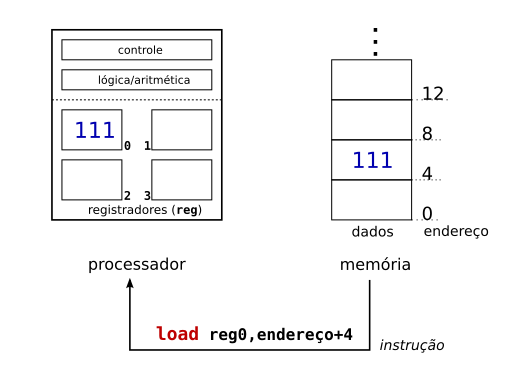
\includegraphics[scale=0.7]{img/instr_mem_load.pdf}}
\only<2>{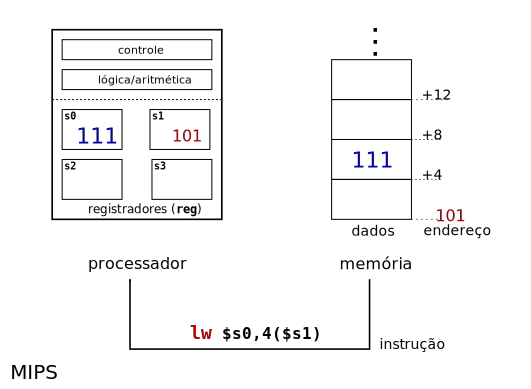
\includegraphics[scale=0.7]{img/instr_mem_load_mips.pdf}}
\end{frame}

\begin{frame}{Operações de memória - \only<1->{{\bf
      Armazenamento}}\only<2>{--MIPS}}{\em \only<1->{{\bf Store}}\only<2>{--MIPS}}
\only<1>{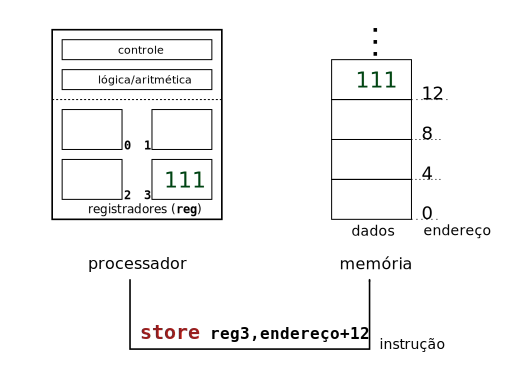
\includegraphics[scale=0.7]{img/instr_mem_store.pdf}}
\only<2>{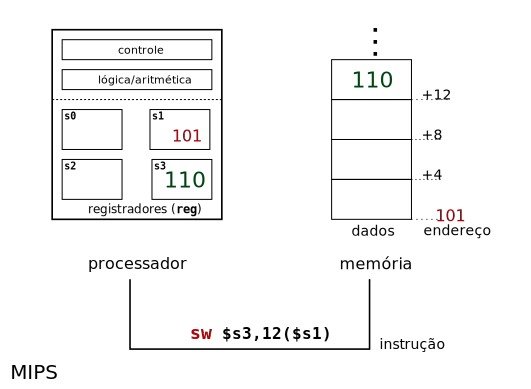
\includegraphics[scale=0.7]{img/instr_mem_store_mips.pdf}}

\end{frame}


\section{Exercícios II}

\def\mem{{\footnotesize\color{gray}\# (M)}}
\begin{frame}{Exercícios II}
  \large

\begin{itemize}
\item Memória
  \begin{enumerate}
  \item $f = g + B[4]$ \mem
  \item $ f = g - A[B[4]]$ \mem
  \end{enumerate}

  \bigskip
  {\footnotesize (M) -- codificar instruções de transferência entre a
    memória e o processador.}
  
\end{itemize}

\end{frame}


\section{Formato das Instruções}

\begin{frame}{Formato básico das instruções MIPS}{Formato R}
  \def\mywidth{1.75cm}
  \def\myheight{0.75cm}

\begin{block}{Formato R (registro)}
  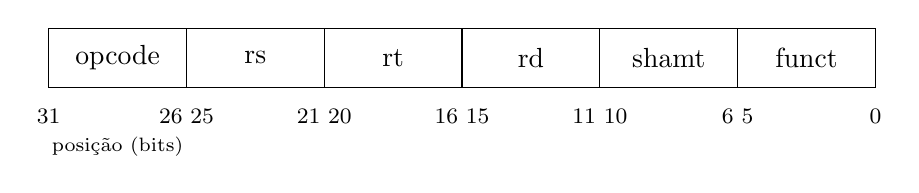
\begin{tikzpicture}
    \foreach \x/\field/\pos in {0/opcode/31,1/rs/{26 25},2/rt/{21
        20},3/rd/{16 15},4/shamt/{11 10},5/funct/{6 5}} {
      \draw (\x*\mywidth,0) rectangle (\x*\mywidth+\mywidth,\myheight);
      \node at (\x*\mywidth+\mywidth/2, \myheight/2) {\field};
      \node at (\x*\mywidth, -\myheight/2) {\footnotesize\pos};
    }
    \node at (6*\mywidth, -\myheight/2) {\footnotesize 0};
    \node at (\mywidth/2, -\myheight) {\scriptsize posição (bits)};
\end{tikzpicture}
\smallskip
\hrule
\bigskip
Exemplo:\\
\begin{tt}
  \hspace{2cm} add \$t0, \$s1, \$s2\\
\end{tt}
{\small\color{gray} \# add -- opcode+funct, rs $\leftarrow$ \$s1, rt
  $\leftarrow$ \$s2, rd $\leftarrow$ \$t0, shamt nulo}\\
\bigskip
  \begin{tikzpicture}
    \foreach \x/\field/\nbits/\ndec in
    {0/\only<1>{000000}/6/\only<2>{\dec{0}},1/\only<1>{10001}/\$s1 -
      5/\only<2>{\dec{17}},2/\only<1>{10010}/\$s2 -
      5/\only<2>{\dec{18}},3/\only<1>{01000}/\$t0 - 5/\only<2>{\dec{8}},4/\only<1>{000000}/5/\only<2>{\dec{0}},5/\only<1>{100000}/6/\only<2>{\dec{32}}} {
      \draw (\x*\mywidth,0) rectangle (\x*\mywidth+\mywidth,\myheight);
      \node at (\x*\mywidth+\mywidth/2, \myheight/2) {\field\ndec};
      \node at (\x*\mywidth+\mywidth/2, -\myheight/2) {\footnotesize\nbits{} bits};
    }
\end{tikzpicture}

\end{block}  

\end{frame}
